\documentclass[a4paper]{article}

\usepackage[T1]{fontenc}
\usepackage{titling}
\usepackage{amsmath}
\usepackage{amsfonts}
\usepackage{graphicx}
\usepackage{mathtools}
\usepackage[includeheadfoot,margin=1in]{geometry}

\usepackage{listings}

\usepackage{chngcntr}
\counterwithin{figure}{section}

\usepackage{caption}
\usepackage{subcaption}

\usepackage{fancyhdr}
\pagestyle{fancy}




\renewcommand{\headrulewidth}{0.5pt}

\numberwithin{equation}{section}
\usepackage[numbered, framed]{matlab-prettifier}

\lstset{
	style              = Matlab-editor,
	escapechar         = ",
	mlshowsectionrules = true,
	tabsize            = 2,
}



\setlength{\droptitle}{-8em}

\title{Homework 3 \\ \large Report}

\author{\textbf{A0153992U, A0000000U, A0000000U} \\ Team ChickenPox}

\date{}

\begin{document}

\maketitle

\section{Introduction}

\subsection{We are awesome}

Hello world!

\section{Feature generation}

Alike image recognition, natural language processing is something that our brains are accustomed to due to millions of years of evolution and fine tuning. We are very good at recognizing the important information and context contained in a written passage, but however natural it may seem, it is certainly not simple to imitate. Given a passage, how can we automatically extract the important information, and how do we connect this to formulate a coherent response?

In order to run machine learning classifiers on the given dataset we decided to play with a number of distinct methods for generating natural language features. Most are based on computing simple statistics such as the number of occurrences on the words or collections of words (bigrams). Some more sophisticated ones tried to also take into account the word order. All are described below.

\subsection{Bag of words}



\subsection{Cantor mapping}

\subsection{Bigrams, Trigrams}

\section{Regularization and validation}

\section{Results}

\section{Improvements}

\begin{figure}[h!]
	\centering
	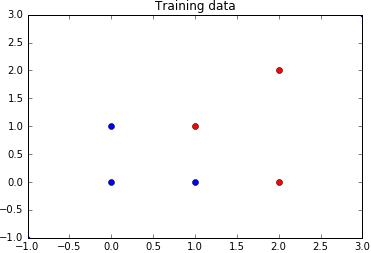
\includegraphics[page=1,width=0.60\textwidth]{diagram.png}
	\caption{\label{fig:diagram}{Hehehe}}
\end{figure}

\begin{lstlisting}[frame=single]
for i:=maxint to 0 do
begin
{ do nothing }
end;
Write('Case insensitive ');
Write('Pascal keywords.');
\end{lstlisting}

\end{document}